\documentclass[format=acmsmall, review=true, screen=true, anonymous=true]{acmart}

\usepackage[english]{babel}

\usepackage{booktabs} % For formal tables

\usepackage[ruled]{algorithm2e} % For algorithms
\renewcommand{\algorithmcfname}{ALGORITHM}
\SetAlFnt{\small}
\SetAlCapFnt{\small}
\SetAlCapNameFnt{\small}
\SetAlCapHSkip{0pt}
\IncMargin{-\parindent}

\usepackage{todonotes}
\usepackage{bookmark}
\usepackage[T1]{fontenc}
\usepackage{microtype}
\usepackage[utf8]{inputenc}

% Metadata Information
%\acmJournal{TWEB}
%\acmVolume{9}
%\acmNumber{4}
%\acmArticle{39}
%\acmYear{2010}
%\acmMonth{3}
%\copyrightyear{2009}
%\acmArticleSeq{9}

% Copyright
%\setcopyright{acmcopyright}
%\setcopyright{acmlicensed}
%\setcopyright{rightsretained}
%\setcopyright{usgov}
%\setcopyright{usgovmixed}
%\setcopyright{cagov}
%\setcopyright{cagovmixed}

% DOI
%\acmDOI{0000001.0000001}

% Paper history
%\received{February 2007}
%\received[revised]{March 2009}
%\received[accepted]{June 2009}

% Document starts
\begin{document}
% Title portion. Note the short title for running heads
\title[Improving credibility and efficiency of decision-making]{Improving credibility and efficiency of decision-making \\ within democratic communities via a statistical quorum}

\author{Mitar Milutinovic}
\affiliation{%
  \institution{UC Berkeley}}
\email{mitar@cs.berkeley.edu}
\author{Maxinder S. Kanwal}
\affiliation{%
  \institution{UC Berkeley}}
\email{mkanwal@berkeley.edu}
\author{David Marn}
\affiliation{%
  \institution{UC Berkeley}}
\email{david.marn@gmail.com}


\begin{abstract}
The Achilles heel of many major democracies is the eternal need for sufficient engagement and attention from the community.
While there have been major efforts towards increasing these attributes within the community, we explore a fundamentally
different approach: For a fixed level of community attention, how can we optimize the allocation of this attention to
maximize productivity?
We propose a novel \textit{statistical quorum}, derived using first principles, as one metric the community can use to
focus attention, in turn making the entire decision-making process dynamic.
We developed a web application centered around this metric and tested it in a 140-person community that holds weekly
councils over the course of 16 weeks.
We found that the community was able to use the web application to simultaneously improve the credibility and efficiency
of their decision-making process.
\end{abstract}


%
% The code below should be generated by the tool at
% http://dl.acm.org/ccs.cfm
% Please copy and paste the code instead of the example below.
%
\begin{CCSXML}
<ccs2012>
<concept>
<concept_id>10003120.10003130.10003131.10003570</concept_id>
<concept_desc>Human-centered computing~Computer supported cooperative work</concept_desc>
<concept_significance>500</concept_significance>
</concept>
<concept>
<concept_id>10003120.10003130.10011764</concept_id>
<concept_desc>Human-centered computing~Collaborative and social computing devices</concept_desc>
<concept_significance>500</concept_significance>
</concept>
<concept>
<concept_id>10010405.10010476.10010936.10003590</concept_id>
<concept_desc>Applied computing~Voting / election technologies</concept_desc>
<concept_significance>500</concept_significance>
</concept>
</ccs2012>
\end{CCSXML}

\ccsdesc[500]{Human-centered computing~Computer supported cooperative work}
\ccsdesc[500]{Human-centered computing~Collaborative and social computing devices}
\ccsdesc[500]{Applied computing~Voting / election technologies}

%
% End generated code
%

\keywords{Decision making; voting; democracy; quorum; credibility; statistical quorum}

\maketitle

% The default list of authors is too long for headers.
\renewcommand{\shortauthors}{M. Milutinovic et al.}

\section{Introduction}

Two of the most shocking democratic votes in recent history occurred in 2016: The referendum vote for Britain to leave the European Union (“Brexit”) and the election of Donald Trump as President of the United States. Both votes were decided by the slimmest of margins, but more significantly, both votes also had poor turnout. The Achilles heel of many major democracies is the eternal need for sufficient engagement and attention from the community. Hence, there have been major efforts towards increasing these attributes within the community. We believe this is a fallacy. Democracy need not suffer under low engagement — in fact, our goal should be to make democracy work with minimal engagement. The ideal governance system is one where citizens do not have to be constantly involved, but the system is still acting as the citizens would like it to.
We explore a fundamentally different approach to making democracy work: \textit{For a fixed level of community attention, how can we optimize the allocation of this attention to maximize productivity?} Can we increase the credibility of decisions made within a democracy while simultaneously skirting the need for an increase in attention? We formulated a novel ‘statistical quorum’, derived using first principles, as one metric the community can use to focus attention, in turn making the entire decision-making process dynamic. We have developed a web application centered around this metric and tested it in a 140-person community that holds weekly councils over the course of 16 weeks. We found that the community was able to use the web application to simultaneously improve the legitimacy and efficiency of their decision-making process.
Our prototyped web application for collective decision-making contrasts with existing similar solutions. Our web application integrates new ideas in how to improve this process: use of \textbf{range voting}, a \textbf{dynamic statistical quorum}, and \textbf{voter delegation}. The broad idea is that, instead of just trying to move the voting process online — something many others have done previously — we in fact wish to add value by voting online. Specifically, we can compute results faster, more accurately, and securely, we can use powerful statistical methods to estimate important quantities for the entire voting population, we can allow for members to entrust their vote to others who have more expertise on specific topics than they themselves do, and we can promote clarity of thought and complete understanding among all members for all voting items.
\textit{Range voting} is voting where members of a community express their positions on open proposals by assigning each a score between –1 and +1. Prior work has shown that this approach generalizes many previous approaches to voting and allows members to express their positions in a highly informative and precise manner. Moreover, if a new proposal is added to a set of existing proposals on which voting was already open, only the new proposal needs to be evaluated by members, as opposed to alternative voting systems where the relative rankings of each proposal would need reassessing.
A \textit{dynamic statistical quorum} uses statistical hypothesis testing to compute the minimum number of required votes needed to achieve a desired level of confidence before a community adopts an outcome as being truly representative of its members’ positions. For example, in a community of 100 members, if 20 members all vote in full support of a proposal, then we can conclude with very high confidence that, had all 100 members actually voted, a majority of them would support the proposal (despite in actuality 80 members having not yet voted). On the other hand, if 80 members vote with 41 voting in favor of the proposal and 39 voting in opposition, then the community cannot yet conclude anything with high confidence (despite the high voter turnout). Hence, the suggested course of action would be for the community to gather more votes and continue discussing the proposal. By utilizing a dynamic statistical quorum, we can direct attention and participation within the community towards contentious proposals, while reducing wasted attention directed towards proposals that already have overwhelming support.
\textit{Voter delegation} addresses two questionable assumptions about current democratic systems: (1) participants have the time to participate and (2) participants have the knowledge to participate. Not all members of a community can participate at all times and not all members have the time to educate themselves about each and every decision being made. By allowing members to define delegates to whom they can give their own vote to — likely those who share their values — their proxy vote can be inferred from their delegates’ votes. In this way, their values are still voiced even if they do not vote directly. If at any point a member decides to vote themselves, then their direct vote is used instead.
All of the above features are combined into a guided process to help community members participate in decision-making. The process starts with a new discussion item where members can comment and discuss a proposal. Moderators then summarize the discussion into three types of points: “in favor,” “against,” and “other”. Members can then use those summaries to help form an opinion before they vote, without having to read every discussion comment made in full detail, thus lowering the barrier of entry into any discussion. As members vote, the app shows the community the average score and confidence in real-time. When the confidence passes a preset threshold, the proposal can be firmly accepted by the community.


In many historical and recent elections it is not infrequent that we get close results (see Table~\ref{tab:example}).
Especially when this is combined with low voter turnout, how can we have confidence in results?
What if elections would be a day longer? What if they would be on a different day? What if
more people would participate? Would results still be the same?

\begin{table}
  \centering
  \begin{small}
  \begin{tabular}{l r r r r r r r}
    {\small\textit{Vote}} & \multicolumn{2}{r}{\small \textit{First option}} & \multicolumn{2}{r}{\small \textit{Second option}} & {\small \textit{Total eligible}} & {\small \textit{Turnout}} & {\small \textit{Decision}} \\
    & & & & & {\small \textit{voters}} & & {\small \textit{credibility}} \\
    \midrule
    Brexit & 17,410,742 & $51.9\%$ & 16,141,241 & $48.1\%$ & 46,500,001 & $72.2\%$ & $59.8\%$ \\
    Presidential elections & 62,984,825 & $48.9\%$ & 65,853,516 & $51.1\%$ & 230,585,915 & $55.9\%$ & $52.6\%$ \\
  \end{tabular}
  \end{small}
  \bigskip\caption{Votes cast in Brexit, a 2016 referendum for United Kingdom's withdrawal from the European Union~\protect\cite{brexitresults},
  and 2016 USA presidential elections, popular vote~\protect\cite{usaresults1,usaresults2}. Simplified to only two options and without
  invalid votes. The last column shows computed decision credibility as described in Section~\ref{sec:decision-credibility}. We see that
  credibility is low, which we can mostly attribute to the fact that there is small difference in votes between both options so with a larger turnout, any option could have ended up winning.}\label{tab:example}
  \vspace{-0.3cm}
\end{table}

An underlying question is what should we do when not everyone in the population votes.

Traditionally, we can have a stance that everyone had an opportunity to vote and express
their preference, so whatever are results based on those who voted are legitimate results.
Research shows, though, that there are many reasons why people do not vote and that there
are many issues related to how elections are organized~\cite{CANCELA2016264, GIMPEL2003471}.

Alternatively, we can see voting as a survey and cast votes as a sample, although imperfect
and non-randomly selected, from a larger population, with a goal to infer the preference
of the whole population. In this setting we can use statistical methods to evaluate the
confidence we can have in the results.

%Moreover, we can see overall participation by everyone in the population as a
%limited resource, a collective attention, we have at our disposal to make collective decisions.
%Traditionally, a common solution to the low voter turnout is to focus on
%increasing the turnout and through that increasing the collective attention available
%for decision making.
%But increasing collective attention for decision making is at odds with other
%demands for the collective and individual attention.
%But once we have a statistical measure of results, we can utilize it to
%optimize the allocation of the collective attention by directing participation towards
%contentious issues.

Our main contributions are:

\begin{enumerate}
\item We developed a framework of computing statistical credibility of results
based on sample size, votes cast, and voting duration.
\item Based on this framework we developed the novel concept of a \emph{statistical quorum} as a threshold of votes required to deem results credible and legitimate.
\item We implement a web application \emph{PeerMind},
integrating credibility of results and statistical quorum, and designed
a workflow of its use in decision making processes.
\item We deployed the application in a democratically run community of 140
members for 16 weeks.
\item Using the analysis of decision making process before and after introduction
of the application, using surveys, and using semi-structured interviews, we show
how use of statistical quorum increases credibility of decisions,
improves utilization of collective attention, increases and diversifies overall participation,
and increases number of decisions made.
\end{enumerate}

The rest of the paper is structured as follows. In Section~\ref{sec:related-work} we
present related work. We continue by describing a framework of computing statistical
credibility of results and statistical quorum in Section~\ref{sec:decision-credibility}.
We present our methodology in Section~\ref{sec:methodology} after which we do
quantitative and qualitative evaluation in Section~\ref{sec:evaluation}. We discuss results in
Section~\ref{sec:discussion} and conclude in Section~\ref{sec:conclusion}. At the end we
have Appendix where we derive formulas presented in Section~\ref{sec:decision-credibility}.

\section{Related Work}
\label{sec:related-work}

%\todo[inline]{Threshold and quorum at \url{https://www.publications.parliament.uk/pa/ld200910/ldselect/ldconst/99/99.pdf}.
%How do some claim that quorum are in fact bad, and counter democratic, but do not offer a solution how to evaluate decisions.}
%
%\todo[inline]{Voting auditing work.}
%
%\todo[inline]{Delegation as way to increase legitimacy, Liquid Democracy, etc.}

%\todo[inline]{Repeat references from "There have been many improvements proposed to this basic form and various analysis made."?}
%
%\todo[inline]{Threshold and quorum at \url{https://www.publications.parliament.uk/pa/ld200910/ldselect/ldconst/99/99.pdf}.
%How do some claim that quorum are in fact bad, and counter democratic, but do not offer a solution how to evaluate decisions.}
%
%\todo[inline]{Voting auditing work.}
%
%\todo[inline]{Delegation as way to increase legitimacy, Liquid Democracy, etc.}
%
%\section{PeerMind Web Application}
%\label{sec:peermind}
%
%\todo[inline]{Something we need to think about is the level of detail we want to go into regarding the implementation/features of PeerMind beyond statistical quorum and range voting.  I think we might want to focus on only those two features for this paper.\\
%I think PeerMind as a comprehensive platform should have its own paper where all of the data is analyzed across the board.  This would be a much more typical HCI paper.  (If I can become president of Ridge in a future semester, we'll have another chance to run a clean, well-designed experiment with a much more developed version of PeerMind.)\\
%The message in the current paper might be clearest if we keep the scope focused on the theory + evaluation/verification.  We should make sure we're not trying to pack too much into one paper.
%\\---Max}
%
%We built a full-fletched real-time web application for collective decision making and voting using Meteor
%framework~\cite{meteor}.
%Users can initiate new discussions which leads them to the main user interface for each discussion as seen
%in Figure~\ref{fig:peermind}.
%
%\begin{figure*}
%  \centering
%  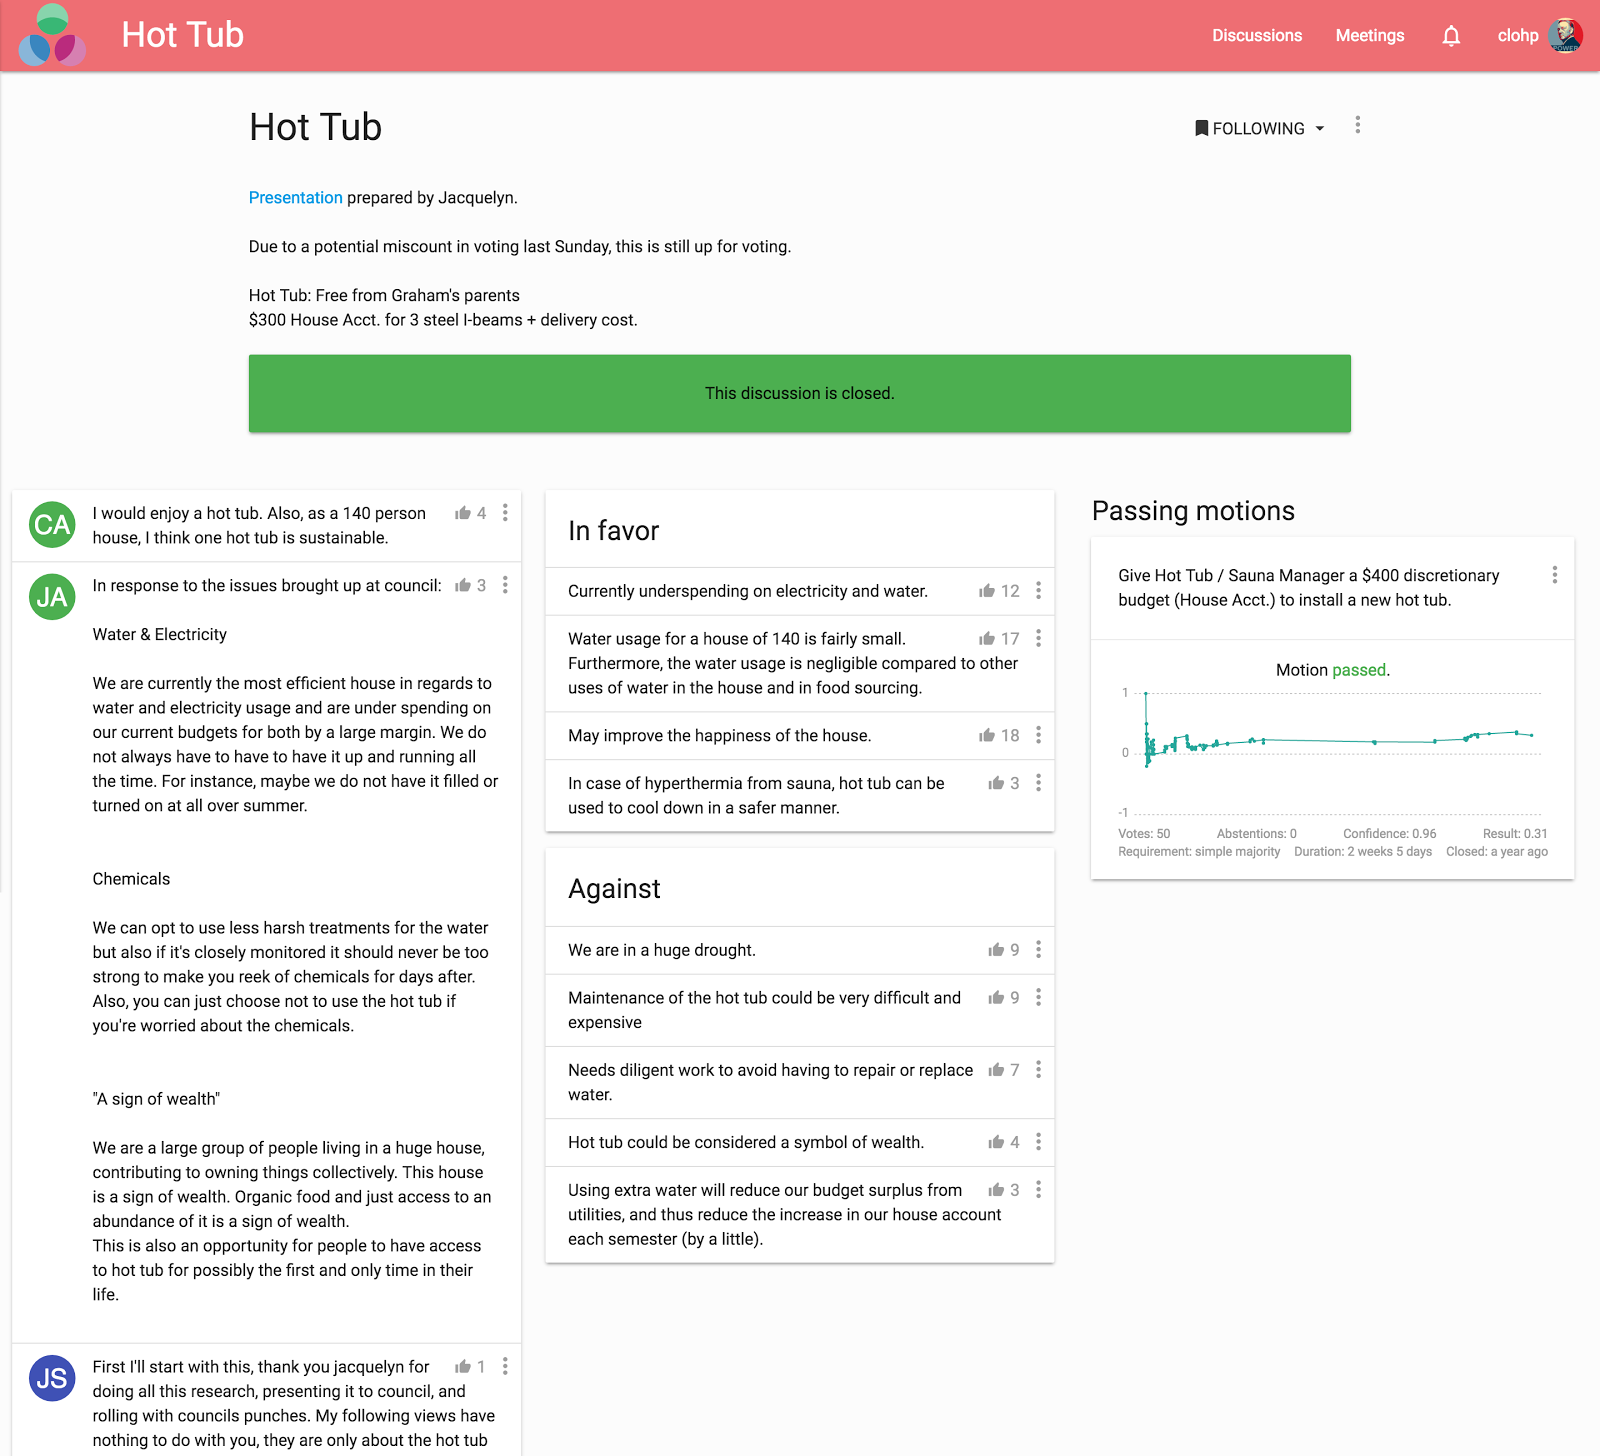
\includegraphics[width=1.75\columnwidth]{figures/peermind.png}
%  \caption{The main PeerMind interface of a discussion. There is initial discussion description on the top and under it there
%  are three columns. A commenting sections for users to discuss it and proposed decisions, a second column where moderators can
%  summarize arguments made during discussion, and a list of proposals to address the discussion.
%  Proposals can be in different states: a proposal being discussed, a proposal being voted on, and with voting concluded.}\label{fig:peermind}
%\end{figure*}
%
%%and discuss them with others online in real-time and with rich-text content.
%%They can attach images and files using drag\&drop. Moderators can summarize discussions into three groups
%
%\todo[inline]{Present how users can see ongoing results during voting. Show an image of active ballot, but with expanded view for current results.}
%
%%Range voting (also known as score voting) is voting where members of a community express their positions on open proposals by assigning
%%each a score on a fixed scale, in the context of this paper, between $-1$ and $+1$.
%%A proposal passes if the average score of all votes on a position is positive.
%%When multiple competing proposals are being voted on, the one with highest average score wins.
%%
%%Prior work has shown that this approach generalizes many previous approaches to voting and allows members to express their
%%positions in a highly informative and precise manner.
%%We find it especially suitable for a web application because many web users are used to use it when ranking products
%%and giving other ``five-star'' feedback.
%%Moreover, if later on a new proposal is added to a set of existing proposals on which voting was already open, only the
%%new proposal needs to be evaluated by members, as opposed to alternative voting systems where the relative rankings of
%%each proposal would need reassessing (assuming members use a consistent personal scale when voting).
%
%\todo[inline]{The app has features both for use in online and offline setting. This allows one to compute
%statistical quorum also for an in-person meeting because math is now more complicated than just counting hands.
%We focus on online experience in this paper.}
%
%\todo[inline]{Security is out of the scope of this work. We assume here that users and their identities are known and are managed
%by a community's admin. There are many communities where their decision making is public with public minutes and this is who
%the app is currently targeting.}

\section{Decision Credibility and Statistical Quorum}
\label{sec:decision-credibility}
A statistical quorum uses statistical hypothesis testing to infer the credibility of the outcome of an open vote before the community adopts the outcome as being truly representative all members' positions.
For example, in a community of 100 members, if 35 members support a specific proposal and 0 oppose, then we can conclude with high probability that, had all 100 members taken the time to vote, a majority of them would be in support of the proposal.  Hence, despite the reality of 65 members not having voted, the outcome of the 35-member vote was credible enough to be taken as representative of the entire community's desire.
On the other hand, if 80 members vote, where 41 support the proposal and 39 oppose, then we cannot yet conclude that the decision to accept the proposal is credible enough for the entire community to officially adopt, despite the significant participation in the vote.
Instead, the suggested course of action would be to continue gathering more votes and/or further discussing the proposal until a credible outcome is established.

By utilizing a statistical quorum, a community can actively direct attention and participation within the community towards contentious proposals, while avoiding wasting attention on noncontroversial proposals.

\subsection{Background}
Consider a community that needs to collectively decide which proposal (if any) to accept out of a set of competing proposals.
To act in democratic fashion, the community may wish to select a winning proposal that either has the support of a \{simple, super\}-majority of all members, or instead is demonstrably preferred over all other competing proposals.  (In some cases, the community may want a winning proposal to satisfy both criteria.)

Ideally, we do not want to poll all members in order to officially accept a proposal, but we do want some level of certainty (e.g., $90\%$ certainty) that
the population is not accidentally accepting an undesired proposal, which in this case encompasses accepting a proposal that is not supported by a majority of members and/or is not clearly preferred over all other competing alternatives.

The primary motivation behind using a statistical quorum is to guarantee a level of credibility before letting a subset of members act on behalf of the entire community.

\subsection{Problem Statement}
We wish to compute the probability that the bias in a community towards supporting a proposal is greater than some
fraction of the population (e.g., $50\%$ for a simple majority, $67\%$ for a super majority).

In addition, we wish to compute the probability that the community bias towards supporting a specific proposal is greater than the community bias towards supporting any competing proposals.

\subsection{Assumptions}
We assume that there is a fixed latent bias for the support of a proposal within the community.  We take each individual vote to be independent and identically distributed (i.i.d.) according to a Bernoulli distribution around this bias.  It should be noted that the independence assumption may not hold in some settings, such as when votes are accumulated over time (one may observe surges of correlated votes).  We will attempt to address this when refining our original formulation of a statistical quorum into a \textit{dynamic} statistical quorum.

Without having collected any votes, we assume that the community's overall bias may be any value between $0\%$ and $100\%$ with equal probability (uniform prior).

\subsection{Voting}

%\url{https://youtu.be/Q60ZXoXP6Hg}

We allow for range voting where each member of the community may choose any real-valued vote $v \in [-1,+1]$ to
represent their vote, with $v = -1$ representing full opposition and $v=+1$ representing full support.  In most applications, it is sensible to quantize $v$ into a fixed number of bins spanning the full range, hence our treatment of $v$ as a discrete random variable.  Because we treat individual votes as a Bernoulli random variable, one can consider $v$ as an individual's average vote.  In the theory subsection below, we rescale $v$ to be in the range $[0,1]$ via the notation $\frac{v + 1}{2}$.

We allow voters to ``abstain'' from voting.
We treat abstentions as indicating that a voter is removing themselves from the community on a given vote.
It is important to distinguish an ``abstention'' (removing one's self from the voting population) from voting $0$ (indicating indifference).

\subsection{Bayesian Theory}

\todo[inline]{Weave in a single concrete example to ground all the abstract theory so that the entire derivation and motivation has a clear and cohesive thread from start to finish.}

\todo[inline]{Hyperparameters: Explain not only what you did, but also why you did it, so that readers (including reviewers) can be convinced that you made appropriate choices.}

After collecting an initial set of votes from members, we want to use that data to construct a prior distribution to help estimate the posterior probability that the proposal is acceptable to the entire community.  Because the sum of  the collected votes follows a binomial distribution, a commonplace and convenient choice for the form of the prior on the community's bias is the Beta distribution (due to its conjugacy with the binomial distribution).  Together, they form the Beta-binomial distribution (also known as the P\'olya urn model).

After extracting the sufficient statistics from raw votes --- namely, the average score and the number of abstentions --- we can adjust the effective community size and corresponding threshold.  In addition, we can calculate the effective number of ``yes'' ($+1$) and ``no'' ($-1$) votes:

Let

\begin{itemize}
\item[$C = $] $\{X_1,\ldots, X_n\}$, the set of competing proposals,
\item[$N = $] population size,
\item[$X_i = $] $\{v_1, \ldots, v_{m_i}\}$, the $m_i$ raw votes for proposal $i$, after excluding abstentions,
\item[$N_i = $] $(N - \textrm{number of abstentions on } X_i)$, the effective population voting on proposal $X_i$,
\item[$\alpha_i = $] $\sum\limits_{v \in X_i}\left(\frac{v+1}{2}\right)$, the effective number of ``yes'' votes on motion $X_i$,
\item[$\beta_i = $] $m_i - \alpha_i$, the effective number of ``no'' votes on motion $X_i$,
\item[$K_i = $] $N_i - m_i$, the number of remaining votes yet to be cast on $X_i$,
\item[$p_i = $] true latent community bias towards voting ``yes'' on $X_i$.
\end{itemize}


In Eqs. \eqref{eq2}, \eqref{eq3}, \eqref{eq5}, \eqref{eq6}, \eqref{eq7} that follow, we urge the reader to refer to the \hyperref[sec:derivation]{Appendix} for complete derivation details, including motivations and justifications.

When considering a single proposal $X_i$ in isolation, we wish to compute:
\begin{align}\label{eq1}
\Pr(\alpha^*_i > T_i \mid X_i),
\end{align}
where
\begin{itemize}
\item[$\alpha^*_i = $] the total number of ``yes'' votes for $X_i$ if we were to sample the entire population,
\item[$T_i = $] $f \cdot N_i$, for some fraction $f$ corresponding to the type of majority needed for the vote
(e.g., $f=\frac{1}{2}$ for a simple majority).
\end{itemize}
Using a desirable prior
\begin{align}\label{eq2}
p_i \mid X_i \sim \operatorname{Beta}(1+\frac{\alpha_i}{K_i},1+\frac{\beta_i}{K_i}),
\end{align}
corresponding to a uniform prior when no votes have been cast ($\alpha_i = \beta_i = 0$), we can express \eqref{eq1} as:
\begin{align}\label{eq3}
\Pr(\alpha^*_i > T_i \mid X_i) &= 1 - {CDF}_{\nu_i}(V_i)
\end{align}
for
\begin{align*}
&\nu_i \sim \operatorname{Beta-Binomial}(1 + \frac{\alpha_i}{K_i}c, 1 + \frac{\beta_i}{K_i}c, K_i),\\
&{CDF}_{\nu_i}(V_i)  = \Pr(\nu_i \leq V_i),
\end{align*}
where
\begin{itemize}
\item[$V_i = $] $\lfloor{T_i - \alpha_i}\rfloor$, the maximum number of additional ``yes'' votes $X_i$ could receive such that it would remain below threshold.,
\item[$c = $] $10$, a hyperparameter chosen by the community based on their relative concern about false alarms versus (temporarily) missed detection.
\end{itemize}

When considering a proposal $X_i$ relative to other proposals in $C$, we wish to compute
\begin{align}\label{eq4}
\Pr\left(\bigwedge_{j \neq i} (\alpha^*_i > \alpha^*_j) \mid C\right)
\end{align}

Under the assumption that the community's votes on motions are independent across motions (which, in many instances, will actually give a lower bound on \eqref{eq3} when a community's support of one proposal is negatively correlated with its support on a competing proposal), we can decompose \eqref{eq3} as follows:
\begin{align}\label{eq5}
& \Pr\left(\bigwedge_{j \neq i} (\alpha^*_i > \alpha^*_j) \mid C\right) = \prod_{j \neq i}\left(1 - \sum_{k=\lceil\delta_{ij}\rceil}^{K_j} \Pr(\nu_j = k) \cdot {CDF}_{\nu_i}(k-\delta_{ij}) \right)
\end{align}
where
\begin{itemize}
\item[$\delta_{ij} = $] $\alpha_i - \alpha_j$, the number of effective ``yes'' votes $X_i$ leads $X_j$ by.
\end{itemize}

Using Eqs. \eqref{eq2} and \eqref{eq4}, we can numerically compute the credibility of a vote's outcome in two key scenarios relevant for democratic communities.  For example, a community may only consider accepting a proposal when a vote's credibility is above $90\%$.

\subsection{Dynamic Statistical Quorum}
Oftentimes, not all proposals are relevant to the entire community.  Instead, a niche proposal may only affect a subset of the community, and hence to require much of the community to indicate their indifference and/or decide their opinion is a waste of the their fixed attentional budget.  While the underlying formulation for a statistical quorum was to establish credibility guarantees before taking action, a natural consequence in common scenarios of the kind just described leads to a reduction in decision-making efficiency.  How can we maintain credibility guarantees while simultaneously boosting efficiency?

Our proposed solution is to infer the \textit{relevant} population size that cares about a given proposal so that we may establish credibility within only the subset population (naturally requiring less global attention).  By replacing the absolute upper bound on this relevant population size ($N_i$) with a high probability upper bound, we can continue to use the same formula presented in Eqs. \eqref{eq2} and \eqref{eq4}, but with more relevant parameters (namely, a smaller $N_i$, which in turn modifies $T_i$, $K_i$, and $V_i$).

To infer $N_i$, we turn to a dynamic voting process whereby information embedded within the dynamics is exploited.  By modeling the arrival rate of new votes as a nonhomogeneous Poisson process, we can extrapolate into the future.  For a decaying arrival rate of new votes, a nonhomogeneous Poisson process $\{N(t),t\geq 0\}$ probabilistically models the number of future arrivals over a given time interval $[0,t)$ according to:
\begin{align*}
\Pr(N(t)=n)={\frac {[\Lambda (t)]^{n}}{n!}}e^{-\Lambda (t)},
\end{align*}
where
\begin{align*}
\Lambda (t)=\int _{0}^{t}\lambda (\tilde{t})\mathrm{d}\tilde{t},
\end{align*}
for some arrival rate process $\lambda (t)$.

For our purposes, we make a natural choice,
\begin{align}\label{eq6}
\lambda (t) = \lambda_0 {(\gamma)}^{\frac{t}{K_i/N_i}},
\end{align}
where
\begin{itemize}
\item[$\lambda_0 =$] a time-averaged rate of vote arrivals (preferably over a unit of time that sufficiently smooths the historical rate),
\item[$\gamma =$] a decay factor ($0 < \gamma < 1$) ideally tuned to fit real historical data for the community via a regression analysis.
\end{itemize}
Now, for example, to upper bound with $95\%$ probability the remaining number of votes still pending, we wish to solve for $\hat{K_i}$ such that the following inequality is satisfied:
\begin{align}\label{eq7}
\lim_{t\rightarrow \infty}\Pr\left(N(t)\leq \hat{K_i}\right) & = \sum_{n=0}^{\hat{K_i}} \frac{\Lambda^n}{n!}e^{-\Lambda} \geq 95\%,
\end{align}
where $\Lambda = \frac{\lambda_0 \cdot K_i/N_i}{\ln{(1/\gamma)}}$.
Upon solving for $\hat{K_i}$, we update $N_i \leftarrow \min\{N_i,\alpha_i + \beta_i + \hat{K_i}\}$, and can proceed to check for a statistical quorum using Eq. \ref{eq5}.

%\begin{figure}[ht]
%\centering
%\includegraphics[width=0.5\textwidth]{figures/}
%\caption{Simple Majority: $\alpha$ vs. $\Pr(\alpha > \frac{1}{2}N)$ for $N=100$, $\beta = 10$.}
%\label{simple_majority}
%\end{figure}

\section{Methodology}
\label{sec:methodology}

To evaluate statistical quorum in practice, we developed a web application PeerMind and
used it in a democratically run community of 140 members for 16 weeks, replacing the traditional
decision making through in-person meetings. The community is a house of 140
students living together and making collective decisions about the governance and operation of
the house, use of resources like common spaces and budgets, and changes to the house itself.

Before the introduction of the application, community had a practice of weekly meetings, councils, with all
members being invited to participate. For decision making it used variation of Robert's rules~\cite{roberts}
with majority and super-majority voting to adopt decisions, generally using hand voting and voice voting.
A fixed quorum of $30\%$ of the membership was used (42 members). Councils generally lasted between one to three hours.
Public minutes were taken.

We introduced the application in fall 2016 semester which lasted 16 weeks. We use spring 2016 semester as
a baseline for comparison, which lasted 16 weeks as well and traditional decision making was used.

To evaluate general perception of members before and after the use of the application for decision making,
we did a general survey at the end of each semester, asking members to answer general questions about the
decision making in the house that semester.

We instrumented the application to collect information on how much time users spent using the application,
measuring the time the application was focused. Other information we used for evaluation are available
through regular features of the application: how many and who made discussion items, comments, proposals
(proposed decisions on discussion items), and vote tallies per proposal.

For the baseline, we extracted similar information from council minutes: how long did the councils last,
how many members participated, how many proposals were proposed and how many passed, and vote tallies for them.

Finally, we did semi-structured interviews after the fall semester with 7 members who were participating
both in spring and fall semesters and ask them to compare their experience between those two semesters and
evaluate the application and the use of statistical quorum.

\subsection{PeerMind}
\label{sec:peermind}

We built a full-fletched mobile-friendly web application using Meteor web framework~\cite{meteor}.
Meteor framework supports reactivity which makes the application update user interface based on actions
of other users in real time. This helps users see comments by other users as they happen, but can also see
progress during voting in real time.

Each user can open and propose new discussion items, which leads them to the main user interface for each discussion as seen in Figure~\ref{fig:peer-mind}, having three sections: commenting section on the left, summary points in the middle,
and proposed proposals with voting on the right. All content inputs fields accept rich text content in WYSWYG manner,
so users can easily add links, images, and other files.

A general workflow after creation of a discussion item is that users discuss it through comments,
which moderators summarize into summary points. At some point an user proposes a proposal which can be
further discussed through comments. Once a moderator deems that proposal is ready to be voted upon
can open it for voting. Users vote through a ballot seen in Figure~\ref{fig:ballot}.

An important design decision in the scope of this paper is that during voting, users can see the current
results of voting in real time. Results are shown on a chart depicting average score through time
as seen in Figure~\ref{fig:results}. Users can see both the current average score of all votes (score
larger than 0 means that a proposal is passing) and the credibility of current result. A community can decide
how high credibility it requires to deem the result passing statistical quorum. During our evaluation
we used 0.90 as statistical quorum.

The rationale for displaying the current results during voting is to give users feedback how voting
is progressing and allow them to engage more with the discussion. Moreover, displaying the results
also serves as additional safeguard against potential manipulations of statistical quorum through malicious
coordination.

After voting passes the statistical quorum, a moderator can close voting and a discussion item.

Web application contains other features which makes it easier to use as a decision making and discusion
platform, like notifications, and additional features which allow the application to be used also to
help run in-person meetings to discuss discussion items made
online. Facilitators of in-person meetings can use it to prepare agendas for meetings, take notes,
and display summary points of current discussion and what proposals are being voted on. Through that the
application can also serve as way to integrate both online and in-person decision making. Having all of
decision making in one platform serves as an important resource for institutional memory.

PeerMind source code is available under open source licence at \url{https://redacted.for.blind.review} and
anonymized dataset of interactions with the app, including votes, is available at \url{https://redacted.for.blind.review}.
The research protocol with human subjects was approved by \emph{redacted for blind review} under
ID \emph{redacted for blind review}.

\begin{figure}[ht]
\centering
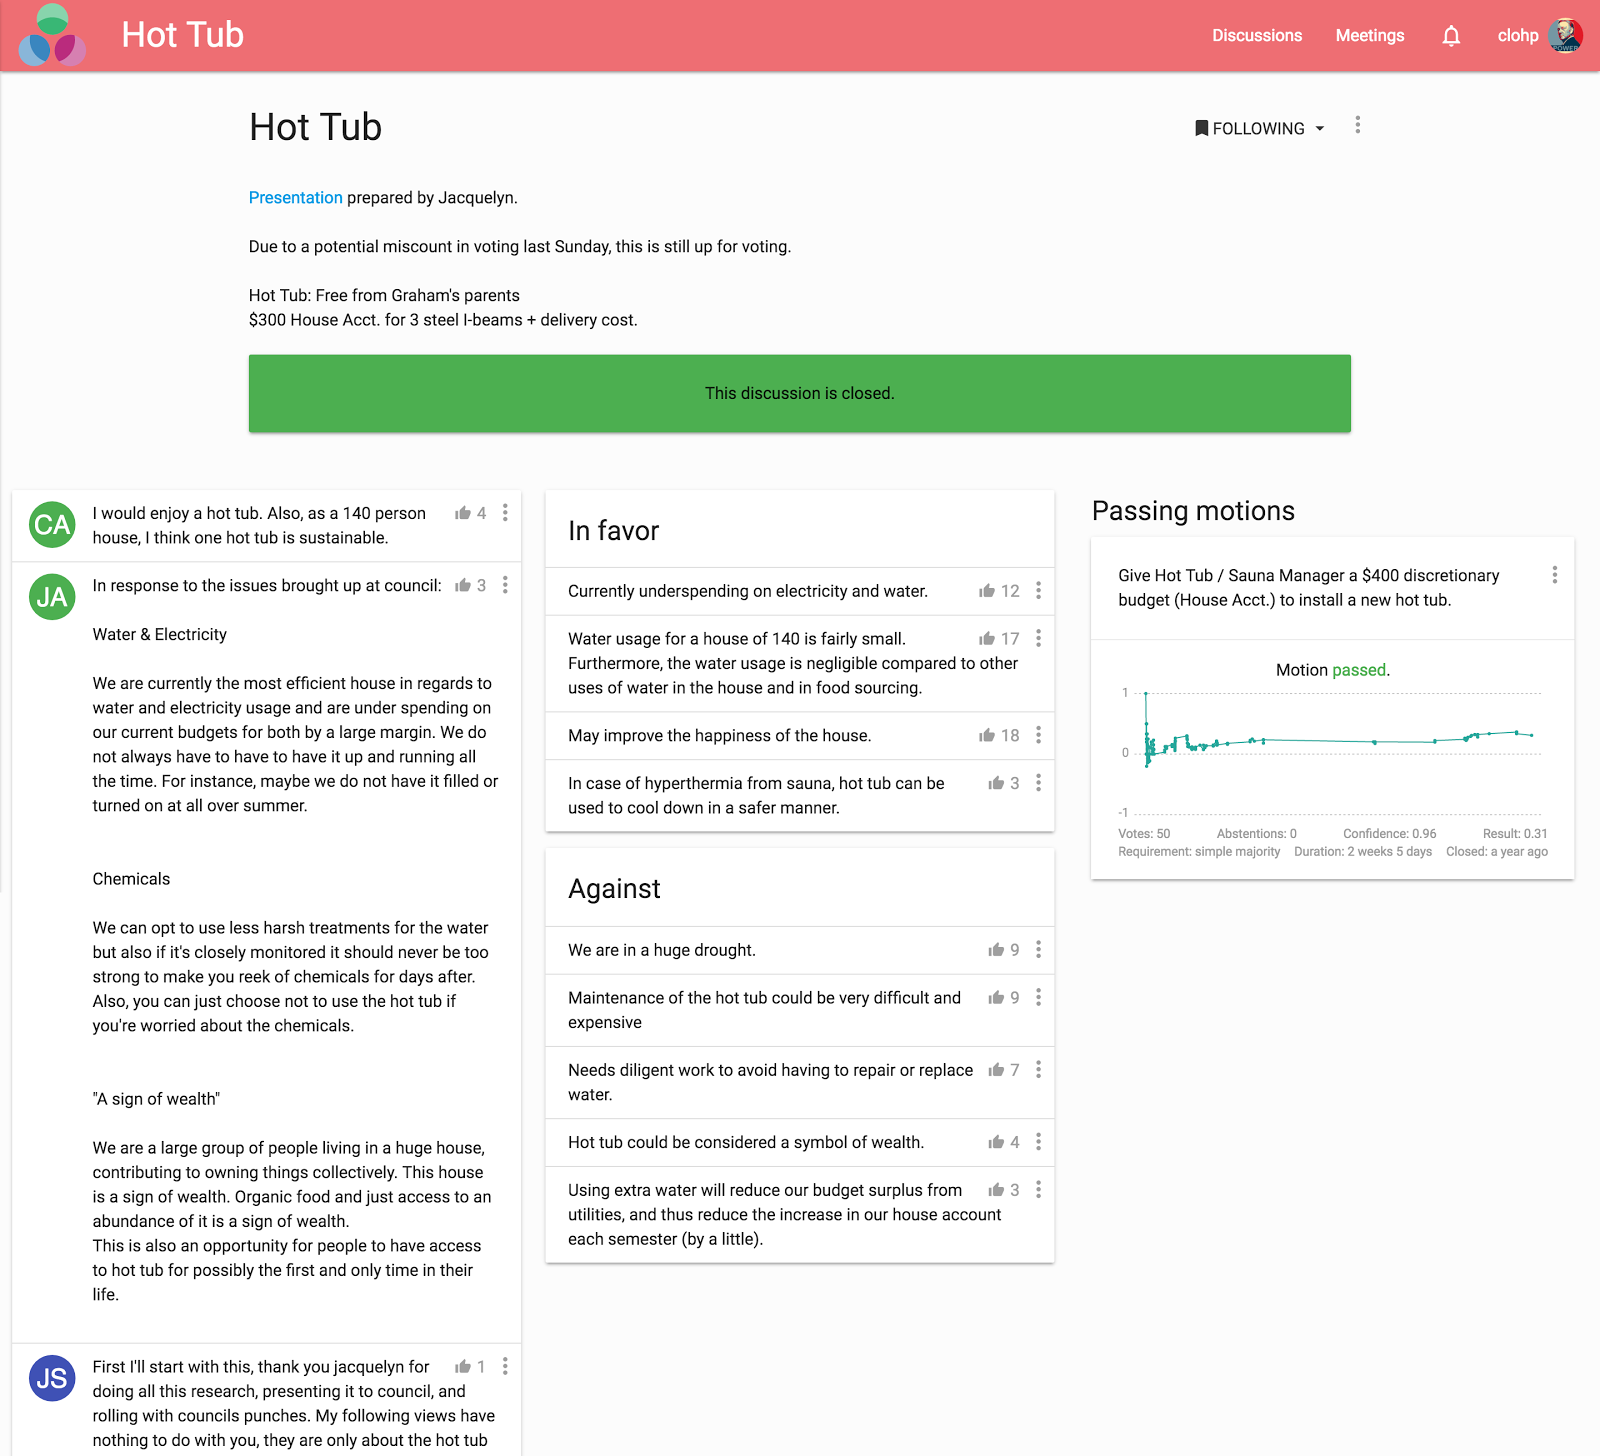
\includegraphics[width=0.9\textwidth]{figures/peermind.png}
\caption{User interface of PeerMind web application. One can see three column structure, with commenting
section on the left, summary points in the middle, and proposed proposals with voting on the right.}
\label{fig:peer-mind}
\end{figure}

\begin{figure}[ht]
\centering
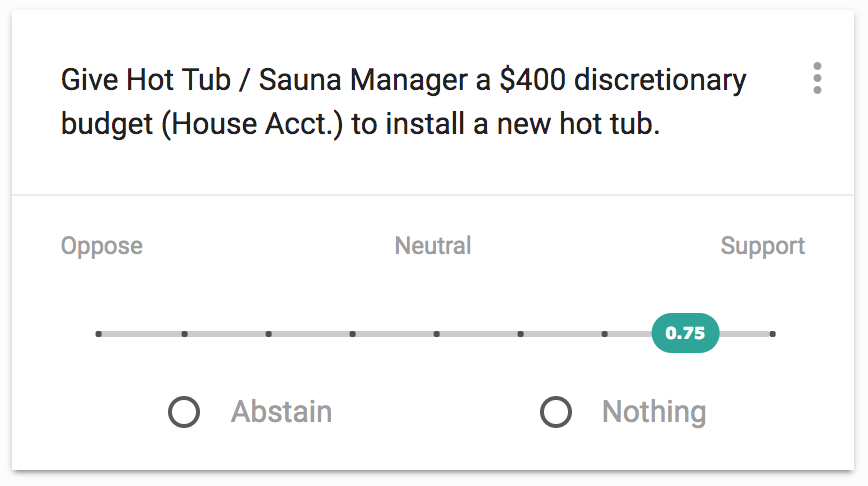
\includegraphics[width=0.5\textwidth]{figures/ballot.png}
\caption{Ballot used for voting in PeerMind web application. Users can chose a value between -1 and 1 on a slider,
where -1 means opposition, 1 means in favor, and 0 indifference. They can also chose abstention (they
remove themselves from the population of the community for voting in question), or to not vote (default), which
means that their vote does not contribute to the quorum.}
\label{fig:ballot}
\end{figure}

\begin{figure}[ht]
\centering
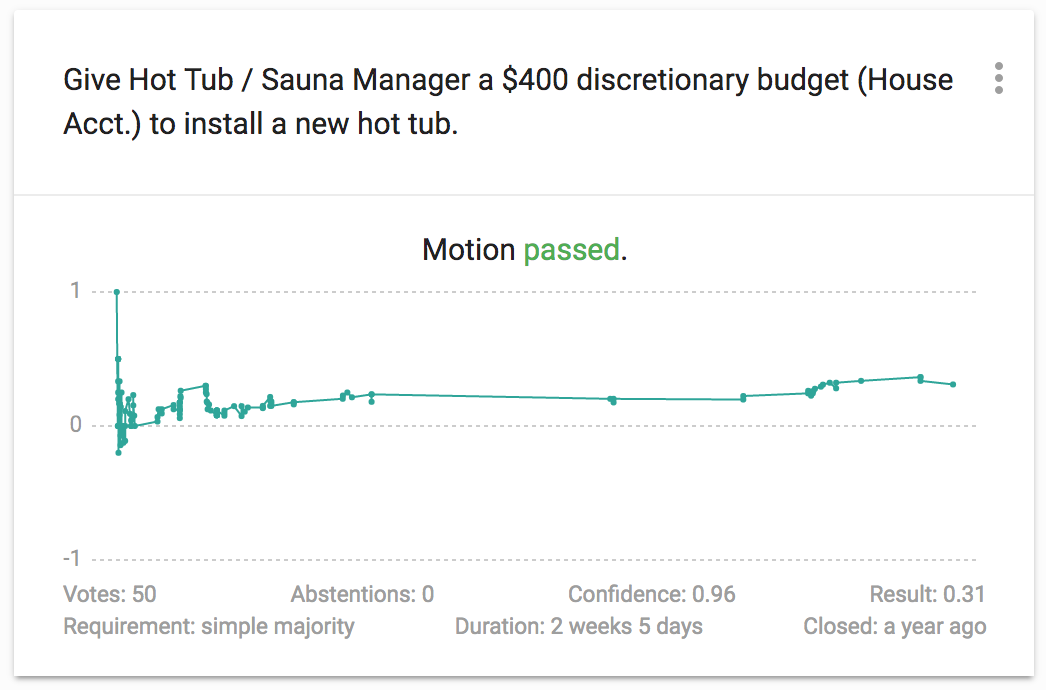
\includegraphics[width=0.6\textwidth]{figures/results.png}
\caption{Results of a vote in PeerMind web application. Results are shown as an average score through time of voting.
A user can hover over the chart to see details at that time. Users can see these results in real time during voting.}
\label{fig:results}
\end{figure}

\section{Evaluation}
\label{sec:evaluation}

We evaluate statistical quorum in two ways. First, we analyze it theoretically and explore its mathematical properties.
Then we do quantitative and qualitative evaluation through real-world use of the PeerMind application by a 140 members
community.

\subsection{Analysis}

\todo[inline]{Visualize the credibility and dynamics of the voting process under this framework:\\
4 Figures and 1 Table Pending}

To gain an intuitive grasp of the decision credibility used in a statistical quorum, we can examine two toy scenarios.

In Figure \ref{fig:credible_interval}, we examine how the $90\%$ credible interval converges as more votes are collected out of a population of $100$.  A statistical quorum is achieved when the credible interval is contained entirely above the x-axis.  In this example, the latent bias of the community is that $75\%$ of the community supports the proposal while $25\%$ opposes it.

In
\begin{figure}[ht]
\centering
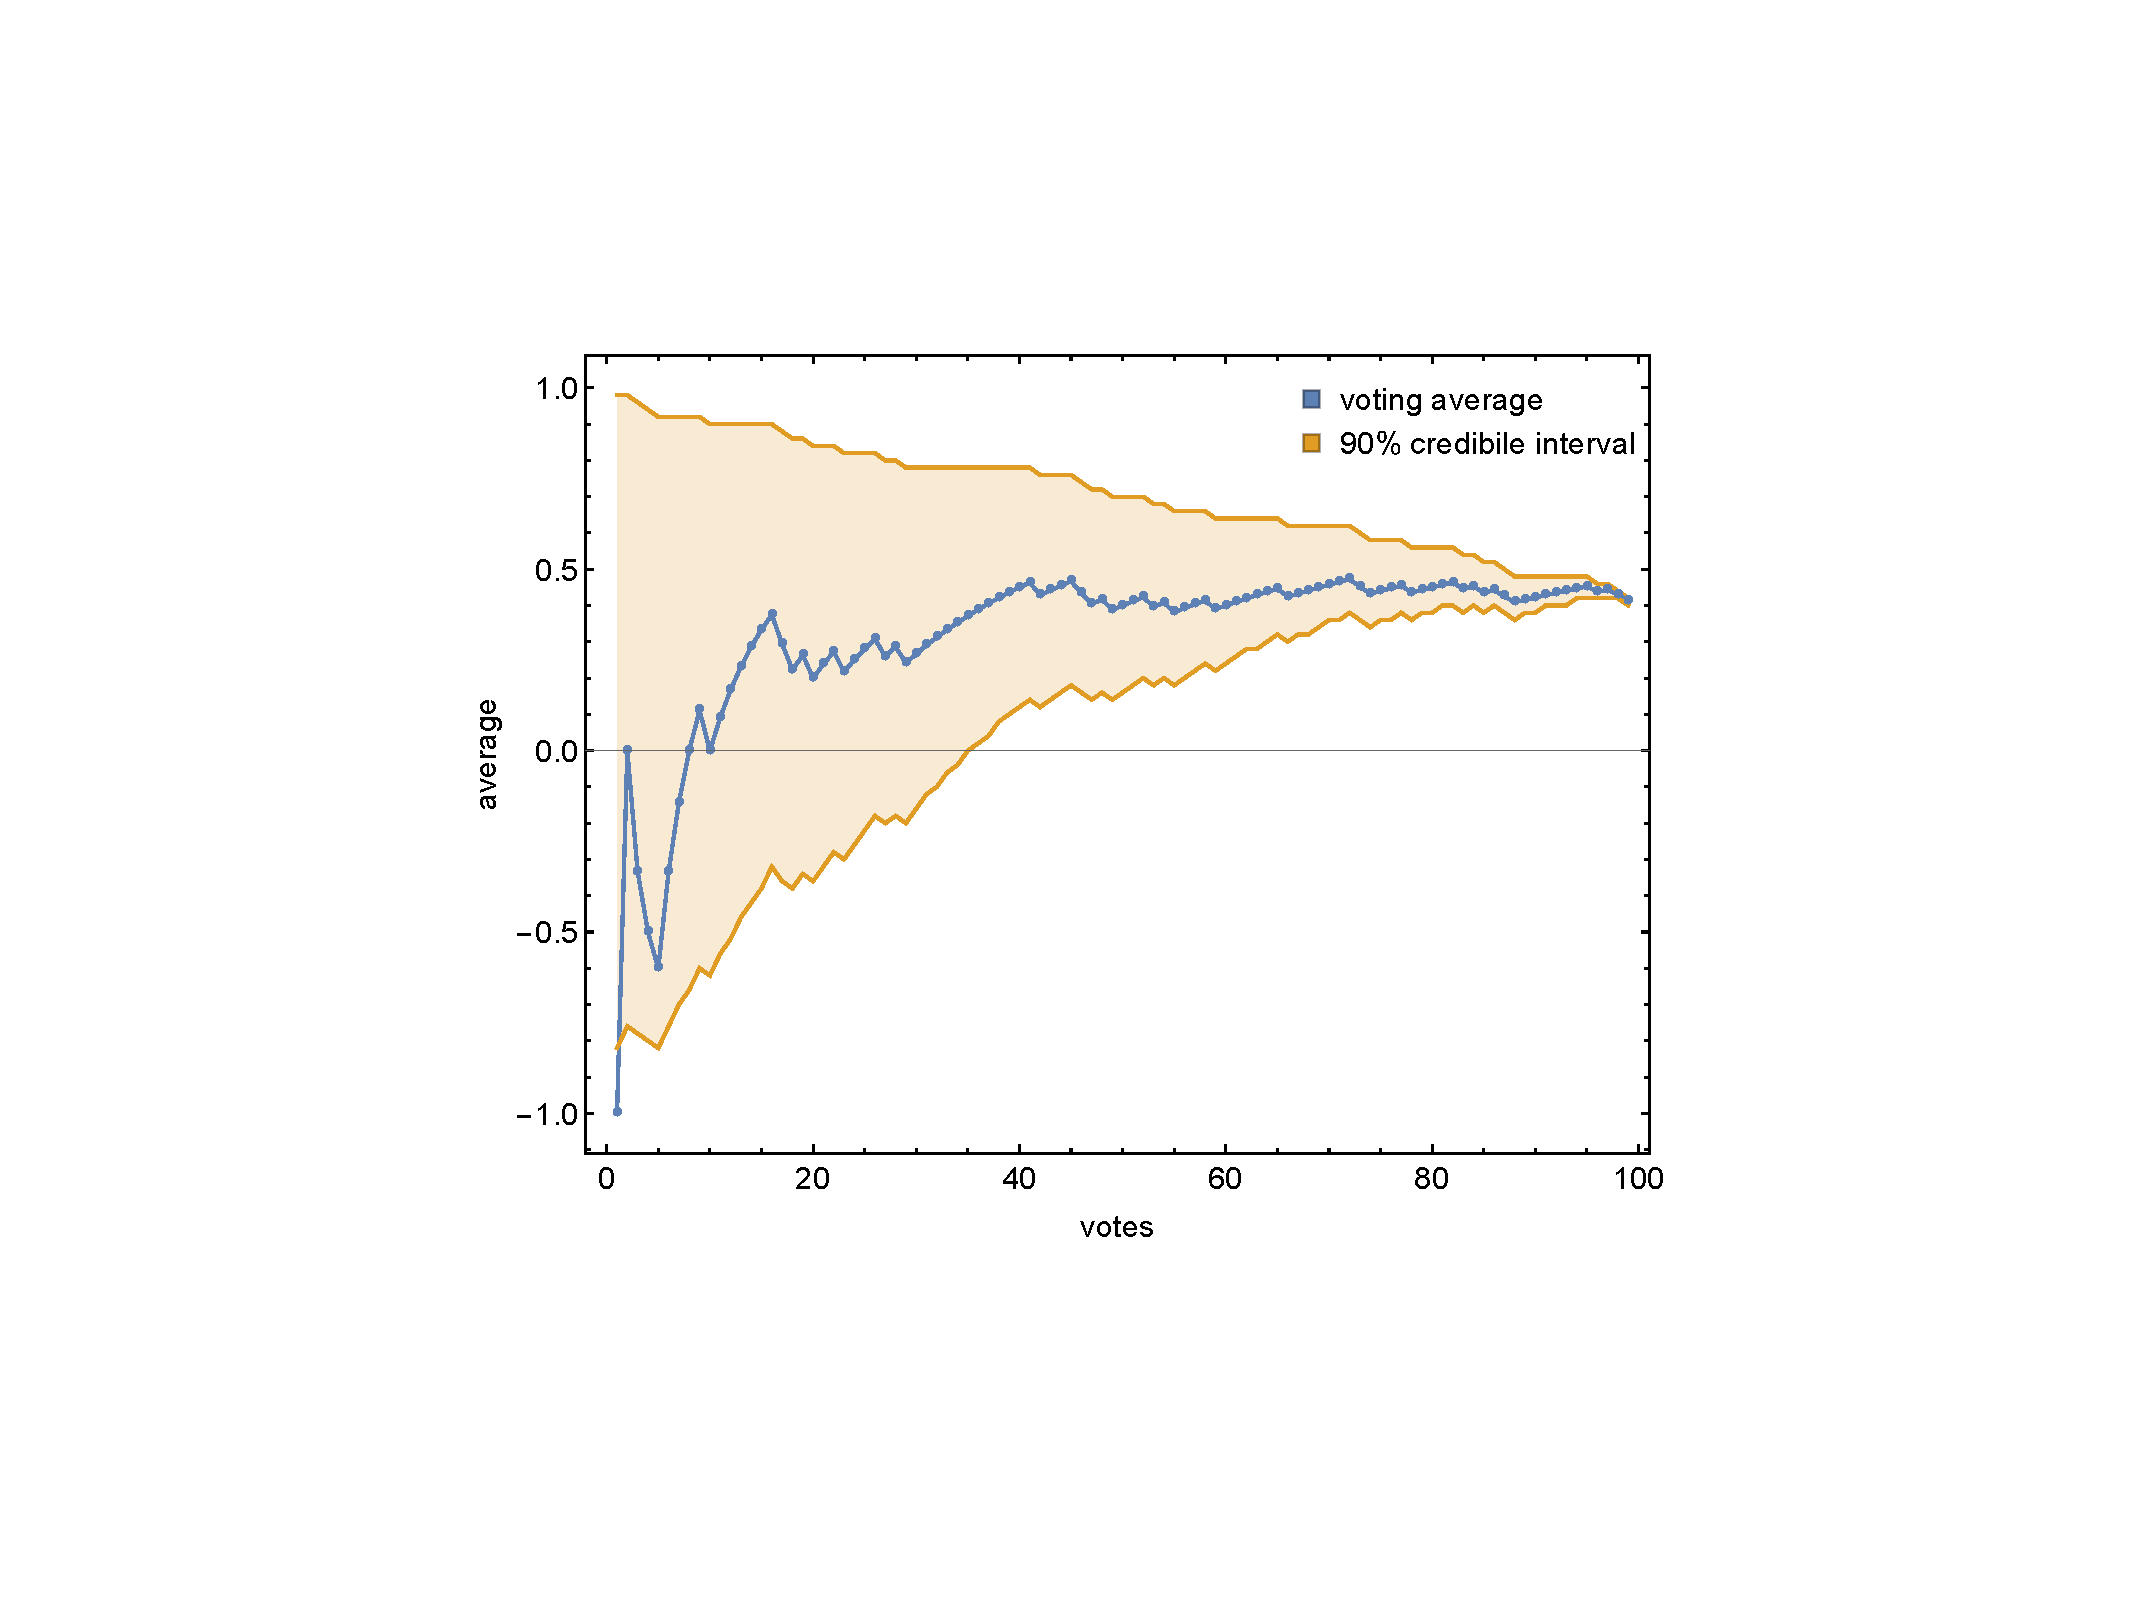
\includegraphics[width=0.45\textwidth]{figures/credible_interval.pdf}
\caption{.}
\label{fig:credible_interval}
\end{figure}

\begin{figure}[ht]
\centering
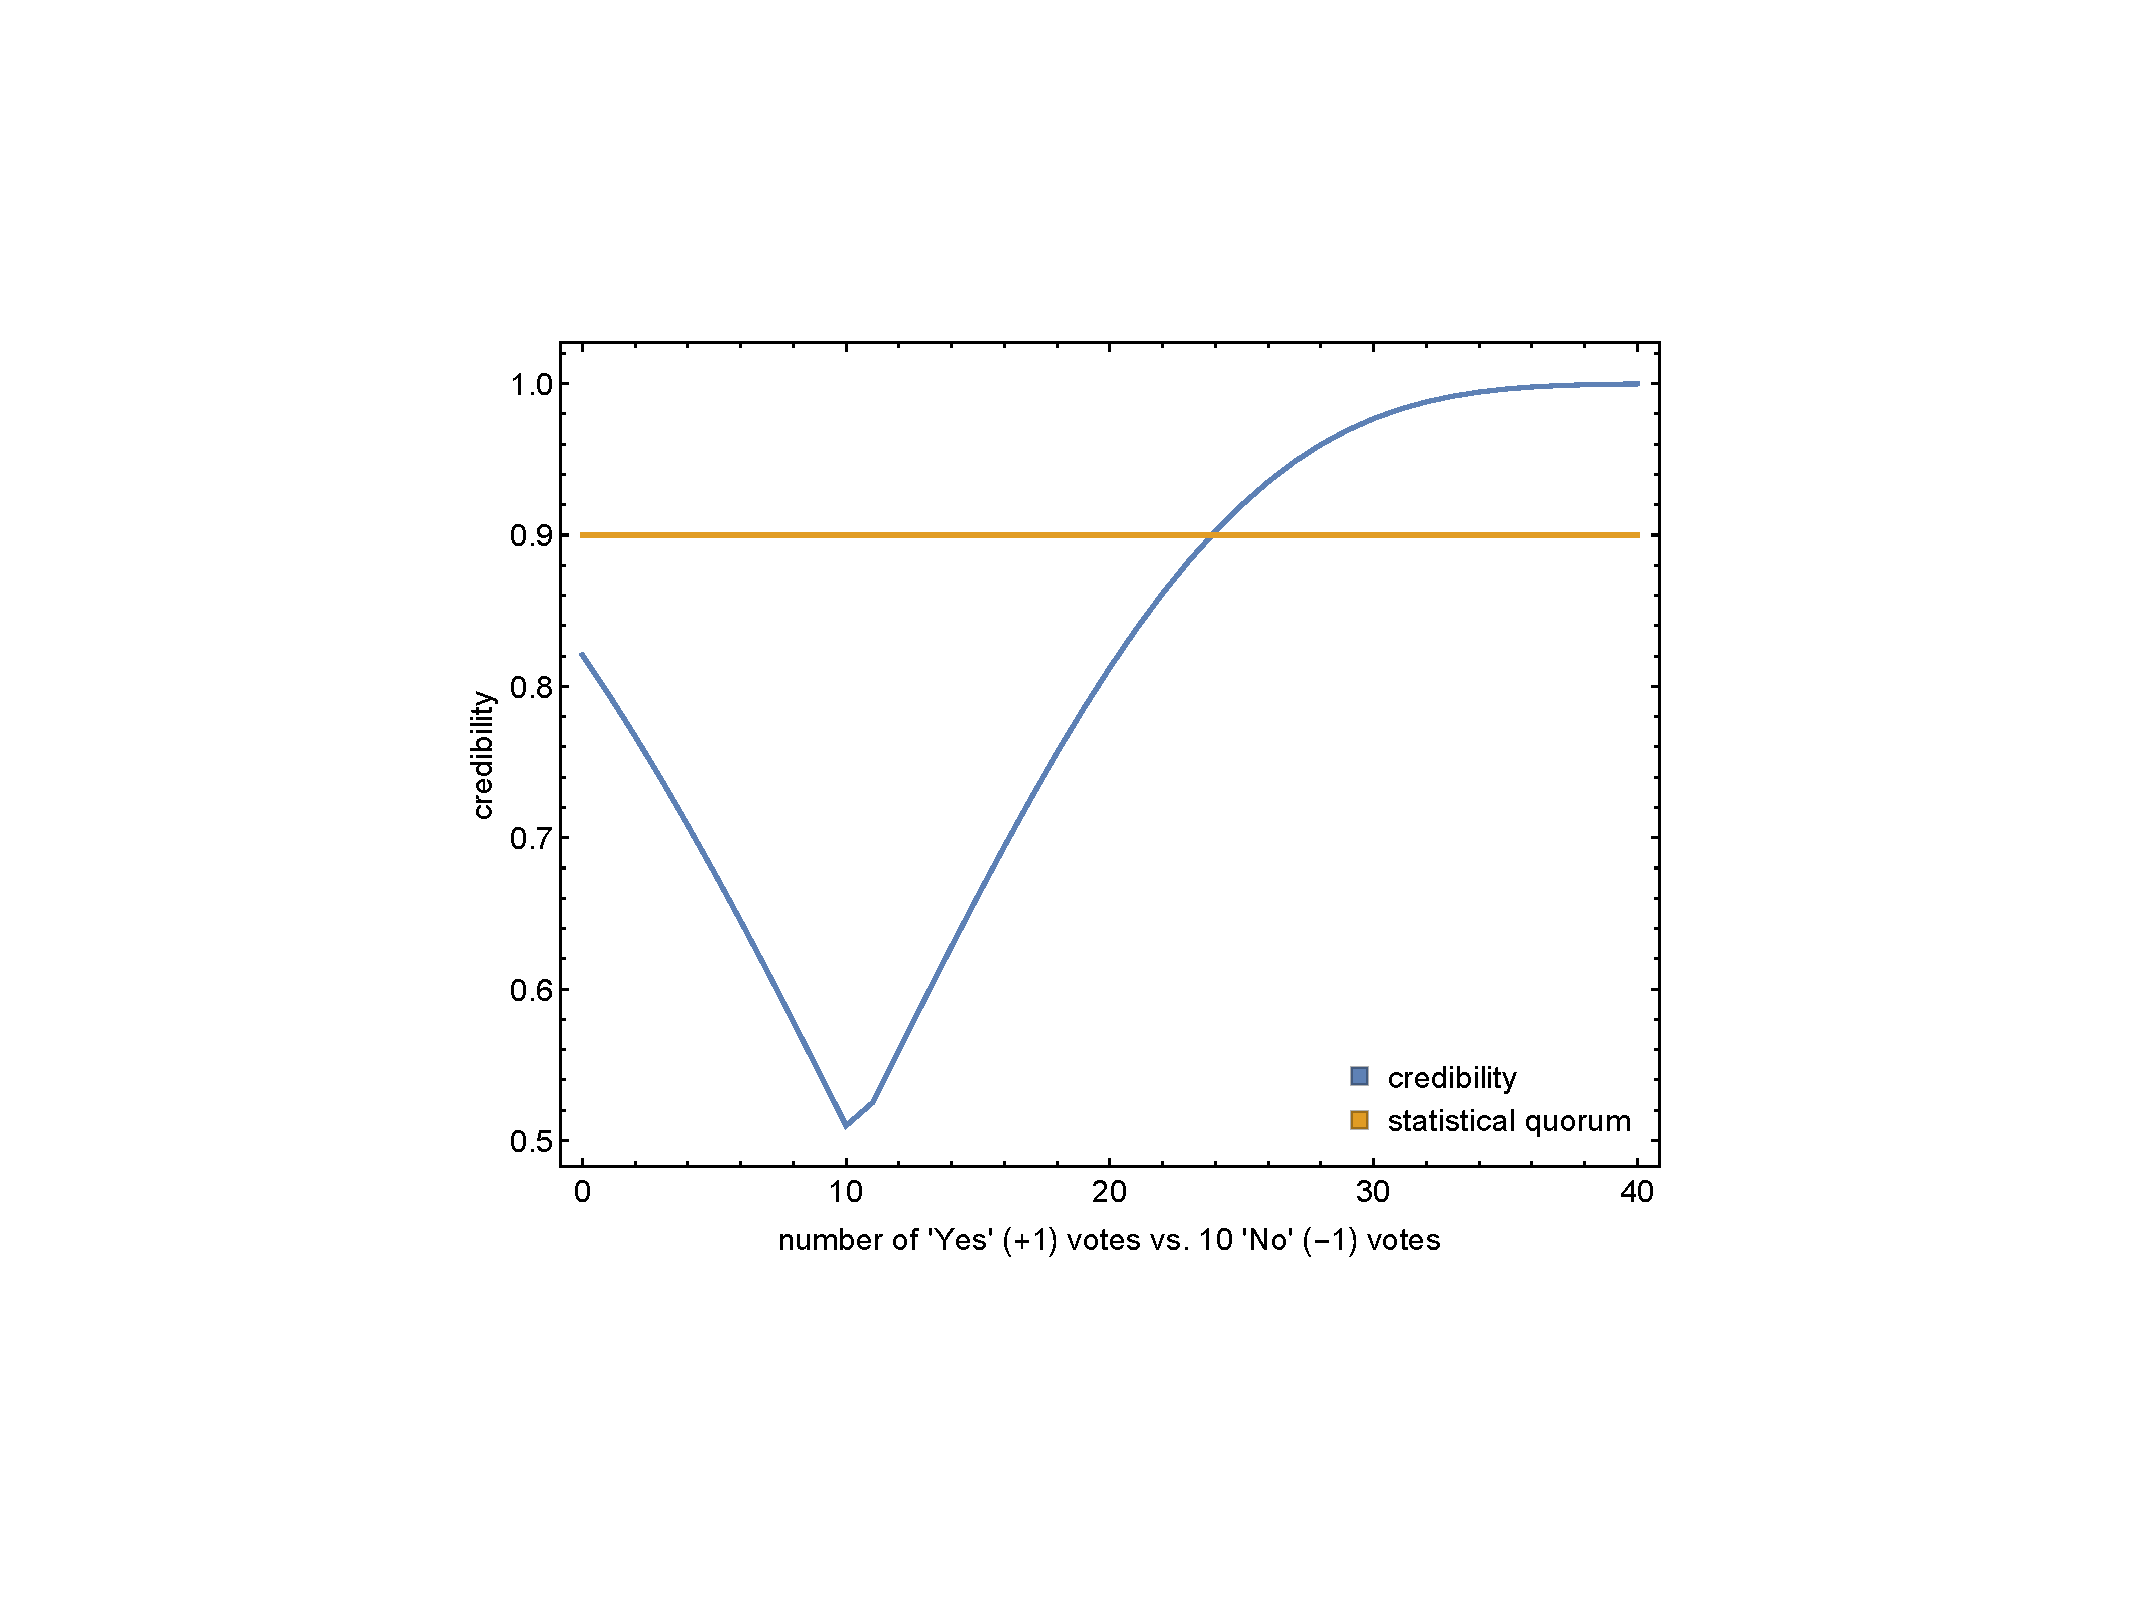
\includegraphics[width=.45\textwidth]{figures/simple_majority.pdf}
\caption{.}
\label{fig:simple_majority}
\end{figure}

\begin{figure}[ht]
\centering
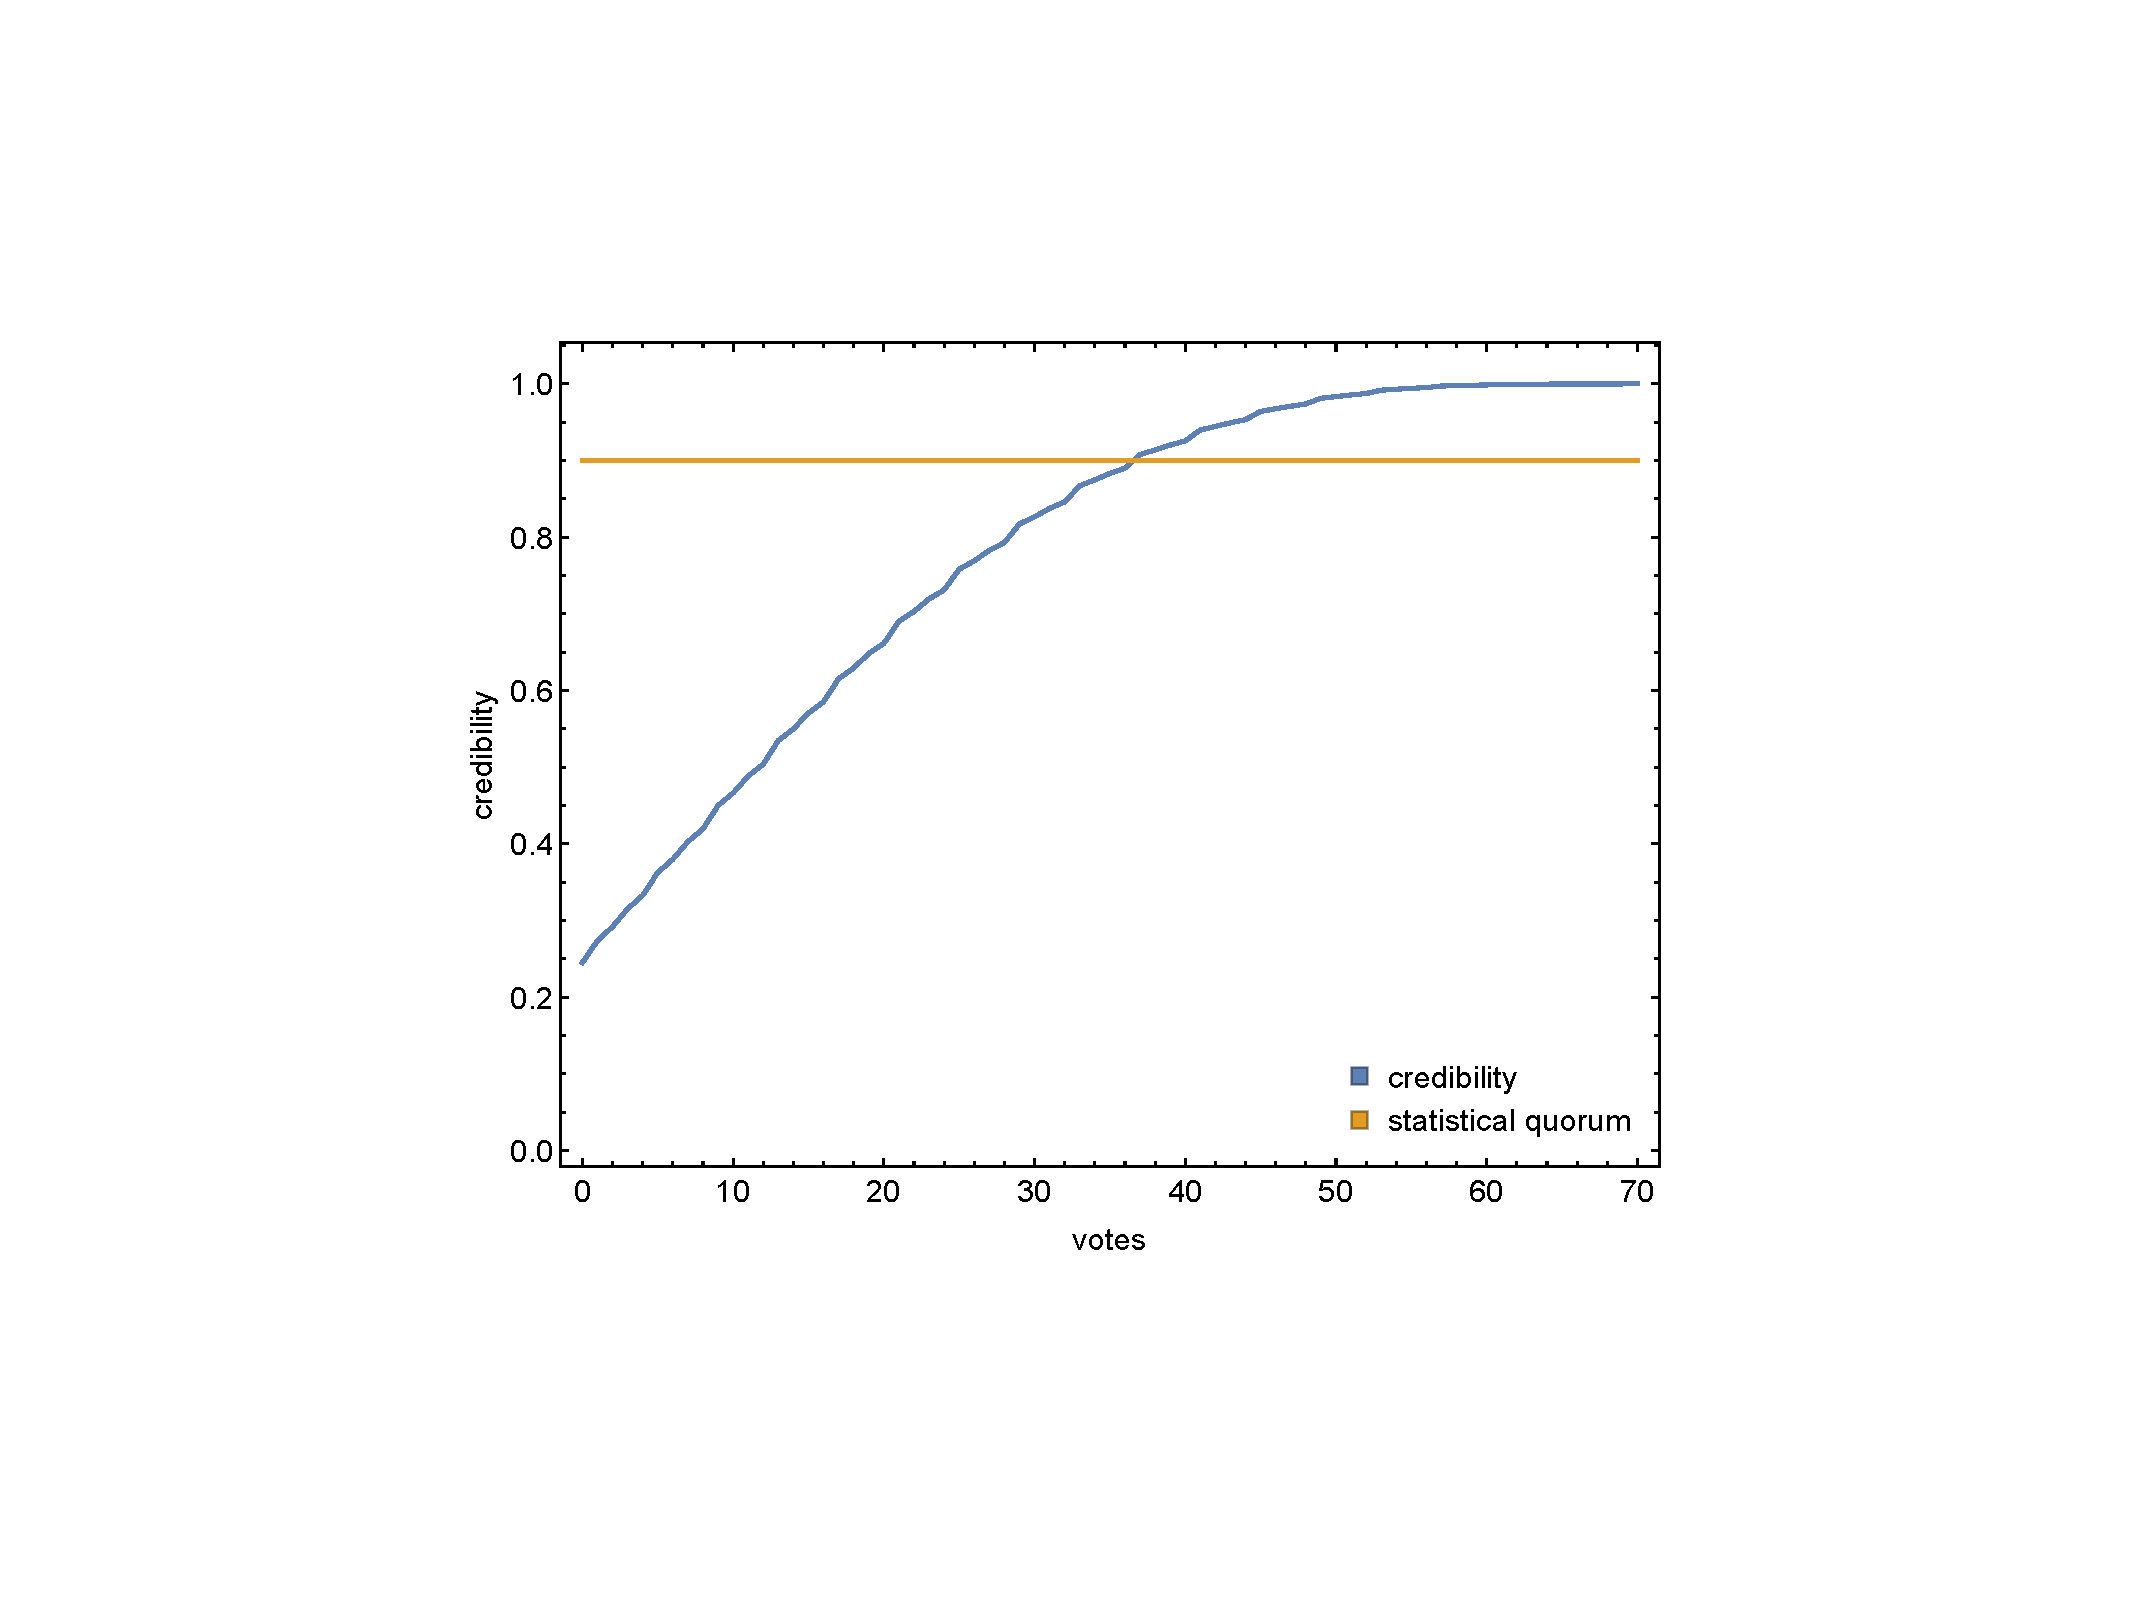
\includegraphics[width=.45\textwidth]{figures/competing_proposals.pdf}
\caption{.}
\label{fig:simple_majority}
\end{figure}


\subsection{Use in Practice}

We tracked web application activity of 132 PeerMind users who consented to the experiment.
We looked at time they had the web application focused in their browsers to determine the
time they used the web application.
In total, they spent 924.886 seconds using the web application (which translates to roughly 2 hours
per member on average) during the fall 2016 semester.

In comparison, we analyzed spring 2016 council minutes when community was meeting in-person and
estimated that members spent approximately 2.600.000 seconds total doing decision making
(around 5 hours per member on average).
We estimated this based on information about beginning and end of councils multiplied
with an estimation of the number of people attending each council.
We estimated the number of people attending based on number of votes made for different proposals
and the quorum size, taking the maximum of both.
We find this a good and conservative proxy because councils have a rule that they have to adjurn
if the number of members present fall under the quorum (42 members) for more than 10 minutes
which in practice members discover soon through the number of votes being made or when count
is explictly requested.

Users on PeerMind made 139 proposals over the span of a semester (this figure
excludes proposals that were withdrawn before voting began).
Out of those 139 proposals, 98 proposals passed. In comparison, 70 out of 73 proposals passed
in the semester prior.

PeerMind users made 3958 votes, whereas 1396 votes were made during spring semester.
Even after adjusting for the larger number of proposals made in the fall, participation
increased significantly.
From around 19 votes per proposal to 28 votes per proposal, on average.



Plotting time spent per user on PeerMind gives further insights into the democratization of decision-making. While the average person spent 7002 seconds on the application, the distribution of users is fairly long-tailed with many people only spending 30 minutes and some people spending upwards of 20 hours. We believe many people who only spent 30 minutes would not participate in the offline council at all (which is confirmed by much lower attendance and fewer votes). Furthermore, people who need more time to discuss are given the freedom to do so without wasting time of those who are not interested in the pertinent discussion.



designed integration with system

minutes and issues with how to get data out



workflow we created -> over one in-person meetings, but because of all decision making happining online, this
didn't happen

issues with quorum
unclear how much time spend on each discussion item: how contentious the discussion really is can be seen only after voting


X people choose not to participate


\todo[inline]{Explain how we were using this for 16 weeks in fall 2016 in a community where traditionally they have
been meeting weekly and now they used it online. How X proposals have been made with Y votes.}

\todo[inline]{Explain how we compare with history: using minutes from spring 2016 for the same community. Issues with
quorum often not bein reached or being lost during the meeting. How many proposals were made then.}

\todo[inline]{Using our metric compare legitimacy of decisions being made in the spring and fall.}

\todo[inline]{We compare how much time collectively was spend on decision making based on minutes in spring 2016 and
how much based on interactions with the platform in fall 2016. Claim is that we made more decisions with less time people
having to be involved in decision making, and with better legitimacy.}

\todo[inline]{We did satisfaction surveys with decision making both in spring and fall 2016. Pull out some interesting
observation when comparing.}

\todo[inline]{Make sure that we are supporting both of our claims well: this statistical quorum is a good metric and
collective attention can be utilized better.}



\subsection{Survey}

In Figure~\ref{fig:survey-comparison} we see questions and results of the survey we made at the end of both semesters.

We can see that in fall (using PeerMind) members were more satisfied with the decision making in the community and only how understandable
is the whole process decreased.

\begin{figure}[ht]
\centering
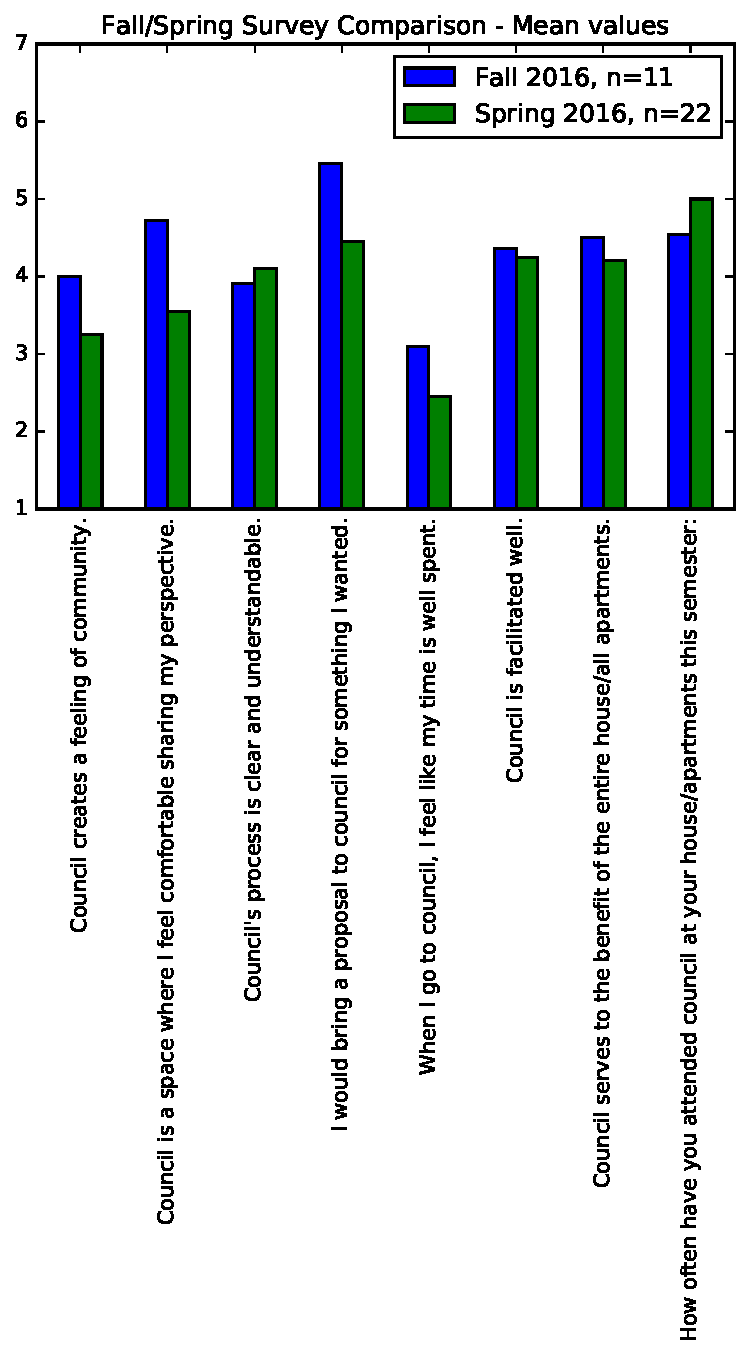
\includegraphics[width=0.9\textwidth]{figures/survey-comparison.pdf}
\caption{Results of a survey at the end of spring (baseline) and fall (using PeerMind) semesters about general perception of the decision making (councils) in the community.
For each question, a participant was asked to rank the answer on a scale between 1 (completely disagree) and 7 (completely agree). All members
of the community were invited to participate in the survey each time.}
\label{fig:survey-comparison}
\end{figure}

\subsection{Interviews}
\label{sec:interviews}

\todo[inline]{We made 7 unstructured interviews. Pull all quotes explaining how they like the idea and how it seems
to work. But how there are other issues by moving decision making online: meetings also serve community building which
does not happen online. No fun. So interesting insights about using online platforms for offline communities
for making decisions which are not really answering our hypothesis, but are useful as insights we got. How some
people prefer online and offline meetings.}

\section{Discussion}
\label{sec:discussion}

decline in understanding of the process:

We attribute this to the fact that the use of the web application is
a novelty, including using a novel concept like statistical quorum, and requires more effort
in educating members than a traditional decision making.
Moreover, decision making in person allows one to observe others how they are participating and
learn from them, instead of being alone using the application.
We explore this question also through interviews in Section~\ref{sec:interviews}.


This not only means that PeerMind users were more productive in terms of decisions made, they also spent significantly less time per motion than the control group.


\todo[inline]{Describe why is $0.90\%$ a reasonable statistical quorum and how to determine one for your community.\\
Part of the answer here is honestly just that the admin should tune the threshold (and a few of the other hyperparameters we introduce) to their intuition.  Once you set the parameters, the real benefit is that you have consistency, rather than having to always use your intuition as an admin about evaluating credibility.}

\todo[inline]{Describe interesting example how we had a bug which were showing a very low statistical quorum for a failing
vote and so the whole community very engaged for a whole month to decide and resolve it. So how they trusted the
app and the metric and how it was really able to direct the attention of the community. It seems it works even if it is
buggy or not perfect, because it has worked so well in the past that members got used to the fact that when it was saying
that there is a consensus or not on an issue that that was also their own read of the community. So for the purpose of
directing attention the metric does not have to mathematically perfect.}

\todo[inline]{Security. How to prevent a group of people to vote and by trick reaching statistical quorum.
We use dynamic statistical quorum to address this, but one other approach is also for voting to stay open and
decisions can then be in the future revoked by people adding more votes, or changing them. But for some decisions
this might not really be possible, because decisions might not be reversible. You can revoke a law, but if you built
a building as a consequence of a decision?\\
(See near/post-quorum validation phase idea in GitHub issues as one suggested solution.)}

\todo[inline]{Discuss how this might or might not lead to a more inclusive decision making: some people prefer it because
they have time to collect thoughts and can participate when they have time, some people do not because they feel
they cannot communicate as effectively, especially with lack of emotions being conveyed.}

%\section{Future Work}
%
%\todo[inline]{More work on security evaluation of potential attacks when a community is using statistical quorum to force a decision.
%Is there a game theoretical approach to it?}
%
%\todo[inline]{How to surface information about credibility to users better than just a number? Visualizations? How can we help them
%understand what exactly this is and how the math works?}

\section{Conclusion}
\label{sec:conclusion}

% Appendix
\appendix
\section*{Appendix}
\label{sec:derivation}

\todo[inline]{Focus on only including bare minimum math, (no ``decorative math'').  Emphasis on justifications and properties, minimal arithmetic.  Good heuristic: Every line of math should have something said about it, otherwise it is unnecessary.}

\subsection*{Derivation of Eq. \eqref{eq2}}
In choosing a Beta prior, we start with $\operatorname{Beta}(1,1)$, as it represents the uniform distribution over all potential values of the community's bias.  To update the prior based on collected votes, standard theory suggests updating to $\operatorname{Beta}(1+\alpha_i,1+\beta_i)$; however, there are a few consistency issues with this update that we seek to fix:
\begin{itemize}
\item[$(1)$] The updated prior should not depend on the absolute number of votes $\alpha_i$, $\beta_i$, as this is not scale-invariant; rather, it should depend on the relative proportions (which are unitless instead of a number of votes),
\item[$(2)$] as $\alpha_i + \beta_i \rightarrow N_i$, $\mathbb{E}[p_i] \rightarrow \frac{\alpha_i}{\alpha_i+\beta_i}$ (at a rate independent of $N_i$),
\item[$(3)$] as $\alpha_i + \beta_i \rightarrow N_i$, $\operatorname{Var}[p_i] \rightarrow 0$ (at a rate independent of $N_i$).
\end{itemize}
To satisfy these consistency properties, we seek to linearly update the prior's scale parameters in a more natural way: $\operatorname{Beta}(1+\eta\alpha_i,1+\eta\beta_i)$ for some renormalizing factor $\eta$.

We can now solve for $\eta$:
\begin{align*}
\operatorname{Var}[p_i] &= \frac{(1+\eta\alpha_i)(1+\eta\beta_i)}{(2+\eta\alpha_i+\eta\beta_i)^2(3+\eta\alpha_i+\eta\beta_i)}
\end{align*}
Clearly, to satisfy $(3)$, we need $\eta \rightarrow \infty$ as $\alpha_i + \beta_i \rightarrow N_i$.  Consequently, the dominant asymptotic term becomes $\frac{1}{\eta^3 (\alpha_i + \beta_i)^3} = \frac{1}{\eta^3 N_i^3}$.  Hence, for the variance to asymptotically approach $0$ at a rate independent of $N_i$, we need $\eta \propto \frac{1}{N_i}$.

Combining these two constraints, we arrive at $\eta \propto \frac{1}{N_i}\cdot \frac{1}{K_i/N_i}$, where the latter factor leads to $\eta \rightarrow \infty$ as $\alpha_i + \beta_i \rightarrow N_i$ without changing the units of $\eta$ ($1/\text{votes}$).

Hence we arrive at $\eta = \frac{c}{K_i}$, where $c$ is any constant that can be selected to tune the rate at which the variance approaches $0$.  In this study, we chose $\eta = \frac{10}{K_i}$ based on the preference of the community.

As a sanity check, one can verify that this form for $\eta$ satisfies properties $(1)-(3)$.

\subsection*{Derivation of Eq. \eqref{eq3}}
\begin{align*}
\Pr(\alpha^*_i > T_i \mid X_i) &= 1 - \Pr(\alpha^*_i \leq T_i \mid X_i), \text{ where}\\
\Pr(\alpha^*_i \leq T_i \mid X_i) &= \int_0^1 \Pr(\alpha^*_i \leq T_i \mid p_i)\cdot \Pr(p_i \mid X_i) \mathrm{d}p_i\\
\end{align*}
Using the binomial and Beta distributions, we get
\begin{align*}
&= \int_0^1 \sum\limits_{v=0}^{V_i} {K_i \choose v} p_i^{v} {(1-p_i)}^{K_i-v} \cdot \operatorname{Beta}(p_i; 1+\frac{\alpha_i}{K_i},1+\frac{\beta_i}{K_i}) \mathrm{d}p_i,\\
&= \sum\limits_{v=0}^{V_i} \underbrace{\int_0^1 {K_i \choose v} p_i^{v} {(1-p_i)}^{K_i-v} \cdot \operatorname{Beta}(p_i; 1+\frac{\alpha_i}{K_i},1+\frac{\beta_i}{K_i}) \mathrm{d}p_i}_{= \Pr(\nu_i = v)\text{ for } \nu_i\ \sim\ \operatorname{Beta-Binomial}(1+\frac{\alpha_i}{K_i},1+\frac{\beta_i}{K_i}, K_i)}.
\end{align*}

Hence, we have
\begin{align*}
\Pr(\alpha^*_1 > T_1 \mid X_1) &= 1 - \sum\limits_{v=0}^{V_i} \Pr(\nu_i = v)\\
&= 1 - \Pr(\nu_i \leq V_i).
\end{align*}

\subsection*{Derivation of Eq. \eqref{eq5}}
Assuming independence of votes across proposals,
\begin{align*}
\Pr\left(\bigwedge_{j \neq i} (\alpha^*_i > \alpha^*_j) \mid C\right) &=\prod_{j \neq i} \Pr(\alpha^*_i > \alpha^*_j \mid X_i, X_j).
\end{align*}
(If, instead, votes in $X_i$ were negatively correlated with votes in $X_j$, and $X_i$ had more support, then the equality ($=$) above would be replaced by an inequality ($>$).)

Further expanding the expression, we get
\begin{align*}
&= \prod_{j \neq i} \left( 1 - \Pr(\alpha^*_i \leq \alpha^*_j \mid X_i, X_j) \right)\\
&= \prod_{j \neq i} \left( 1 - \sum_{k=\lceil\delta_{ij}\rceil}^{K_j} \underbrace{\Pr(\alpha^*_j = \alpha_j + k \mid X_j)}_{= \Pr(\nu_j = k)} \cdot \underbrace{\Pr(\alpha^*_i \leq \alpha_j + k \mid X_i)}_{={CDF}_{\nu_i}(k - \delta_{ij})} \right).
\end{align*}

\subsection*{Derivation of Eq. \eqref{eq6}}
The properties we desire for $\lambda(t)$ are:
\begin{itemize}
\item[$(1)$] as $K_i \rightarrow 0$, the rate of incoming votes should drop exponentially and should be independent of $N_i$,
\item[$(2)$] as $t \rightarrow \infty$, the rate of incoming votes should drop exponentially.
\end{itemize}
Setting $\lambda (t) = \lambda_0 {(\gamma)}^{\frac{t}{K_i/N_i}}$ for $0 < \gamma < 1$ satisfies these constraints while still allowing for the exact rate to be tunable.

\subsection*{Derivation of Eq. \eqref{eq7}}
Using $\lambda (t) = \lambda_0 {(\gamma)}^{\frac{t}{K_i/N_i}}$, we have
\begin{align*}
\lim_{t \rightarrow \infty} \Lambda (t) &=\int _{0}^{\infty}\lambda (t)\mathrm{d}t\\
&= \int _{0}^{\infty} \lambda_0 {(\gamma)}^{\frac{t}{K_i/N_i}} \mathrm{d}t\\
&= \lambda_0 \frac{K_i/N_i}{\ln{(1/\gamma)}}.
\end{align*}
Thus,
\begin{align*}
\lim_{t\rightarrow \infty}\Pr\left(N(t) = n\right) = \frac{(\lambda_0 \cdot K_i/N_i)^n}{n!(\ln{(1/\gamma)})^n}e^{-\lambda_0 \frac{K_i/N_i}{\ln{(1/\gamma)}}},
\end{align*}
and
\begin{align*}
\lim_{t\rightarrow \infty}\Pr\left(N(t)\leq \hat{K_i}\right) & = \sum_{n=0}^{\hat{K_i}} \frac{(\lambda_0 \cdot K_i/N_i)^n}{n!(\ln{(1/\gamma)})^n}e^{-\lambda_0 \frac{K_i/N_i}{\ln{(1/\gamma)}}}.
\end{align*}

%\begin{acks}
%\end{acks}

% Bibliography
\bibliographystyle{ACM-Reference-Format}
\bibliography{refs}

\end{document}
